\documentclass[12pt]{article}
\usepackage[svgnames,x11names,table]{xcolor}
\usepackage{hyperref}
\usepackage{graphicx}
\usepackage{parskip}
\usepackage{float}
\usepackage{amsmath}
\usepackage{esint}
\usepackage{amssymb}
\usepackage{enumitem}
\usepackage[thicklines]{cancel}

\hypersetup{
    colorlinks,
    citecolor=blue,
    filecolor=black,
    linkcolor=black,
    urlcolor=RoyalBlue4,
}

\title{PEU 218 Assignment 5}
\author{Mohamed Hussien El-Deeb (201900052)}
\date{\today}

\DeclareMathOperator{\sech}{sech}
\DeclareMathOperator{\csch}{csch}

\begin{document}

\maketitle
\tableofcontents
\hypersetup{linkcolor=RoyalBlue4}

\newpage
\section{Question 1}

\subsection{Problem}

Use the Divergence theorem to evaluate \(\iint_S \vec{F} \cdot d \vec{S}\) where \(\vec{F}=\sin (\pi x) \hat{\imath}+z y^3 \hat{\jmath}+\left(z^2+4 x\right) \hat{k}\) and \(S\) is the surface of the box with \(-1 \leq x \leq 2,0 \leq y \leq 1\) and \(1 \leq z \leq 4\). Note that all six sides of the box are included in \(S\).

\subsection{Solution}

\[
    \iiint_V \vec{\nabla} \cdot \overrightarrow{\boldsymbol{u}} d V=\oiint_S \overrightarrow{\boldsymbol{u}} \cdot \widehat{\boldsymbol{n}} d S
\]

\[
    \vec{\nabla} \cdot \vec{F} =
    + \pi \cos (\pi x)
    + 3 z y^2
    + 2 z
\]

\[
    \iiint_V \vec{\nabla} \cdot \vec{F} d V
    = \int_{1}^{4} \int_{0}^{1} \int_{-1}^{2} \left( \pi \cos (\pi x) + 3 z y^2 + 2 z \right) d x d y d z
\]

\[
    = \int_{1}^{4} \int_{0}^{1} {\left[ \sin (\pi x) + 3 z y^2 x + 2 z x \right]}_{-1}^{2} d y d z
\]

\[
    = \int_{1}^{4} \int_{0}^{1} \left( 6 z y^2 + 4 z \right) d y d z
\]

\[
    = \int_{1}^{4} {\left[ 2 z y^3 + 4 z y \right]}_{0}^{1} d z
\]

\[
    = 6 \int_{1}^{4} z d z
    = 3 {\left[ z^2 \right]}_{1}^{4}
    = 3 \left( 16 - 1 \right)
    = 45
\]

\newpage
\section{Question 2}

\subsection{Problem}

Use Stokes' theorem to evaluate \(\int_C \vec{F} \cdot d \vec{r}\) where \(\vec{F}=\left(3 y x^2+z^3\right) \hat{\imath}+y^2 \hat{\jmath}+4 y x^2 \hat{k}\) and \(C\) is the triangle with vertices \((0,0,3),(0,2,0)\) and \((4,0,0)\). \(C\) has a counter clockwise rotation if you are above the triangle and looking towards the \(x y\)-plane. See the figure below for a sketch of the curve

\begin{figure}[H]
    \centering
    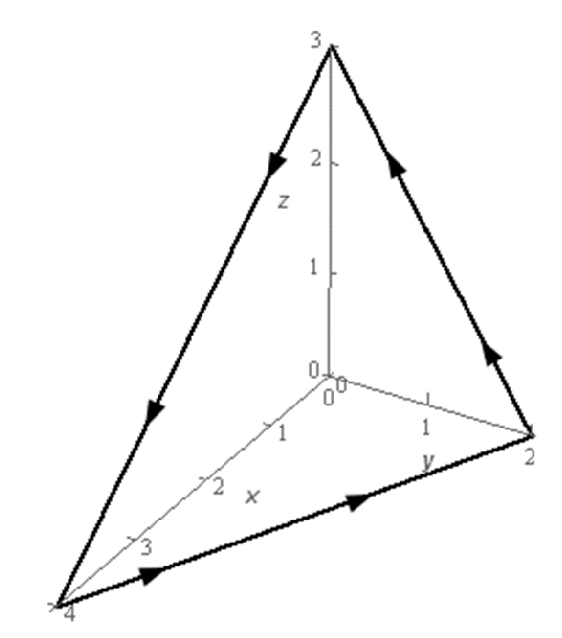
\includegraphics[width=0.5\textwidth]{Q2.png}
\end{figure}

\subsection{Solution}

\[
    \iint_S \vec{\nabla} \times \overrightarrow{\boldsymbol{u}} \cdot \widehat{\boldsymbol{n}} d S=\oint_C \overrightarrow{\boldsymbol{u}} \cdot d \vec{r}
\]

\[
    \vec{\nabla} \times \vec{F} =
    \begin{vmatrix}
        \hat{\imath}                & \hat{\jmath}                & \hat{k}                     \\
        \frac{\partial}{\partial x} & \frac{\partial}{\partial y} & \frac{\partial}{\partial z} \\
        3 y x^2 + z^3               & y^2                         & 4 y x^2
    \end{vmatrix}
    = 4 x^2 \hat{\imath} + \left(3 z^2 - 8 x y\right)  \hat{\jmath} - 3 x^2 \hat{k}
\]

The normal of the triangle is same as the normal of the plane that passes through the three vertices of the triangle.

The equation of the plane is

\[
    \frac{x}{4} + \frac{y}{2} + \frac{z}{3} = 1
\]

The normal of the plane and the triangle is

\[
    \vec{n} = \left( \frac{1}{4}, \frac{1}{2}, \frac{1}{3} \right)
\]

\[
    \hat{n} = \frac{\vec{n}}{\left| \vec{n} \right|}
    = \frac{\frac{1}{4} \hat{\imath} + \frac{1}{2} \hat{\jmath} + \frac{1}{3} \hat{k}}{\sqrt{\frac{1}{16} + \frac{1}{4} + \frac{1}{9}}}
    = \frac{3 \hat{\imath} + 6 \hat{\jmath} + 4 \hat{k}}{\sqrt{61}}
\]

\[
    \vec{\nabla} \times \vec{F} \cdot \hat{n}
    = \left(
    4 x^2 \hat{\imath}
    + \left(3 z^2 - 8 x y\right) \hat{\jmath}
    - 3 x^2 \hat{k}
    \right) \cdot
    \frac{3 \hat{\imath} + 6 \hat{\jmath} + 4 \hat{k}}{\sqrt{61}}
\]

\[
    = \frac{12 x^2 + 18 z^2 - 48 x y - 12 x^2}{\sqrt{61}}
    = \frac{18 z^2 - 48 x y}{\sqrt{61}}
\]

\[
    \iint_S \vec{\nabla} \times \vec{F} \cdot \hat{n} d S
    = \frac{6}{\sqrt{61}} \iint_S \left(3 z^2 - 8 x y\right)  d S
\]

\[
    \iint_S f(x, y, z) d S= \iint_D f(x, y, g(x, y))|\vec{\nabla} \emptyset| d x d y
\]

\[
    g(x, y) = 3 - \frac{3}{4} x - \frac{3}{2} y
\]

\[
    \emptyset = z - 3 + \frac{3}{4} x + \frac{3}{2} y
\]

\[
    \vec{\nabla} \emptyset = \left( \frac{3}{4}, \frac{3}{2}, 1 \right)
\]

\[
    |\vec{\nabla} \emptyset| = \sqrt{{\left( \frac{3}{4} \right)}^2 + {\left( \frac{3}{2} \right)}^2 + 1^2}
    = \sqrt{\frac{9}{16} + \frac{9}{4} + 1}
    = \sqrt{\frac{9 + 36 + 16}{16}}
\]

\[
    = \sqrt{\frac{61}{16}}
    = \frac{\sqrt{61}}{4}
\]

\[
    \iint_S \vec{\nabla} \times \vec{F} \cdot \hat{n} d S
    = \frac{3}{2} \int_0^2 \int_0^{4-2y} \left(\frac{27}{16} {\left(x + 2y - 4\right)}^2 - 8 x y\right)  dx dy
\]


\[
    = \frac{3}{2} \int_0^2 {\left[\frac{27}{48} {\left(x + 2y - 4\right)}^3 - 4 x^2 y\right]}_0^{4-2y} dy
\]

\[
    = - \frac{3}{2} \int_0^2 {\left(16 {\left(y-2\right)}^2 y + \frac{27}{6} {\left(y - 2\right)}^3\right) } dy
\]

\[
    = - \frac{3}{2} \int_0^2 {\left(16 \left(y^3-4y^2+4y\right) + \frac{27}{6} {\left(y - 2\right)}^3\right) } dy
\]

\[
    = - \frac{3}{2} {\left[16 \left(\frac{y^4}{4}-\frac{4}{3}y^3+2y^2\right) + \frac{27}{24} {\left(y - 2\right)}^4\right] }_0^2
\]

\[
    = - \frac{3}{2} \left(16 \left(\frac{16}{4}-\frac{32}{3}+8\right) - \frac{27*16}{24}\right)
\]

\[
    = - 5
\]

\newpage
\section{Question 3}

\subsection{Problem}

Evaluate the line integral

\[
    I=\oint_C\left[y\left(4 x^2+y^2\right) d x+x\left(2 x^2+3 y^2\right) d y\right]
\]

around the ellipse \(\frac{x^2}{a^2}+\frac{y^2}{b^2}=1\)

\subsection{Solution}

\[
    \oint_C P d x+Q d y=\iint_R\left(\frac{\partial Q}{\partial x}-\frac{\partial P}{\partial y}\right) d x d y
\]

\[
    P = y\left(4 x^2+y^2\right), \quad Q = x\left(2 x^2+3 y^2\right)
\]

\[
    \frac{\partial Q}{\partial x} = 6x^2 + 3 y^2, \quad \frac{\partial P}{\partial y} = 4 x^2 + 3 y^2
\]

\[
    \frac{\partial Q}{\partial x} - \frac{\partial P}{\partial y} = 2 x^2
\]

\[
    \iint_R 2 x^2 d x d y
    = 2 \int_{-b}^{b} \int_{-a \sqrt{1 - \frac{y^2}{b^2}}}^{a \sqrt{1 - \frac{y^2}{b^2}}} x^2 d x d y
\]

\[
    = \frac{2}{3} \int_{-b}^{b} {\left[ x^3 \right]}_{-a \sqrt{1 - \frac{y^2}{b^2}}}^{a \sqrt{1 - \frac{y^2}{b^2}}} d y
    = \frac{4}{3} a^3 \int_{-b}^{b} {\left(1 - \frac{y^2}{b^2}\right) }^\frac{3}{2} d y
    = \frac{\pi}{2} a^3 b
\]

\newpage
\bibliographystyle{plain}
\bibliography{references}
\nocite{El-Deeb_PEU-218_Assignments}

\end{document}